\documentclass[12pt]{article}

%packages
\usepackage{graphicx}
\usepackage{amsmath}
\usepackage{mathdots}
\usepackage{amsthm}
\usepackage{amssymb}
\usepackage{fancyhdr}
\pagenumbering{arabic}
\usepackage{hyperref}
\usepackage{lscape}
%Margins etc...
\setlength{\textheight}{240mm}
\setlength{\topmargin}{-17mm} \setlength{\oddsidemargin}{-4mm}
\setlength{\textwidth}{166mm} \setlength{\parindent}{0mm}
\setlength{\marginparsep}{9mm} \setlength{\parskip}{3mm}

\begin{document}
\begin{center}
\Huge{Exploring Mixed Strategies with Sage - Solution\\\tiny{This sheet was last updated \today.} }
\end{center}




\begin{enumerate}
\item Modify the input to consider the following game:
\begin{center}
\begin{tabular}{|c|c|}
\hline
$7,3$&$4,1$\\\hline
$1,2$&$6,4$\\
\hline
\end{tabular}
\end{center}
\item If player 1 is using the mixed strategy: $\rho=(.3,.7)$, what is player 2's best response?\\
Graphically it is immediate to see that if $\rho=(.3,.7)$ then player 2's best response is $\sigma=(0,1)$.
\begin{center}
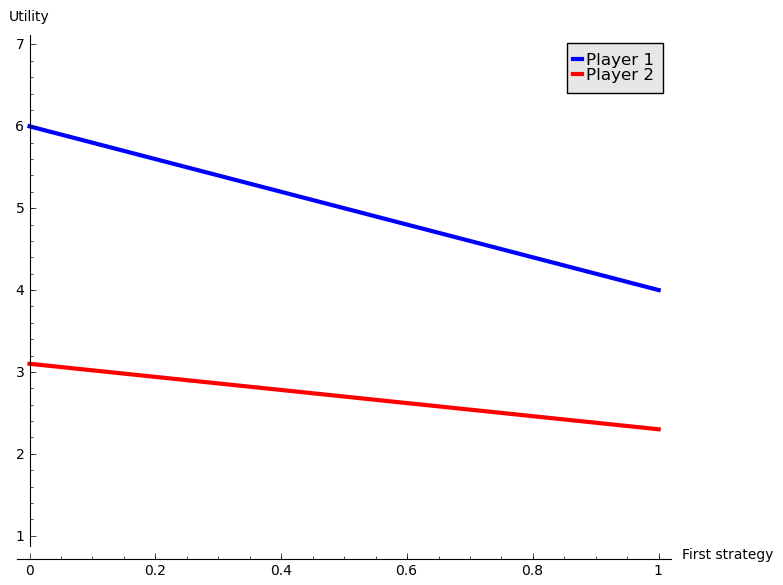
\includegraphics[width=8cm]{sage15.png}
\end{center}
Analytically we see that:
$$u_2((.3,.7),(q,1-q))=q(.3\times3+.7\times2)+(1-q)(.3\times1+.7\times4)=-.8q+3.1$$
which is a decreasing function and as such is maximised for $q=0$.
\item What are the equilibria strategies?\\
The interact tells us that the equilibria are at:
$$((1,0),(1,0))$$
$$((0,1),(0,1))$$
$$\left(\left({1\over2},{1\over2}\right),\left({1\over4},{3\over 4}\right)\right)$$
The first two equilibria are easy to find by identifying best responses. The 3rd equilibria can be found using the equality of payoffs theorem and solving the following system of equations:

$$7\times q+4\times(1-q)=1\times q+6\times(1-q)$$
$$3\times p+2\times(1-p)=1\times p+4\times(1-p)$$
which simplifies to:

$$8q=2$$
$$4p=2$$
As required.
\item What are the expected utilities to both players at each equilibria?
The 2 pure strategy equilibria gives utilities:
$$u_1=7\text{ and }u_2=3$$
$$u_1=6\text{ and }u_2=4$$
respectively. The utilities at the third equilibria can be seen to be:

\begin{center}
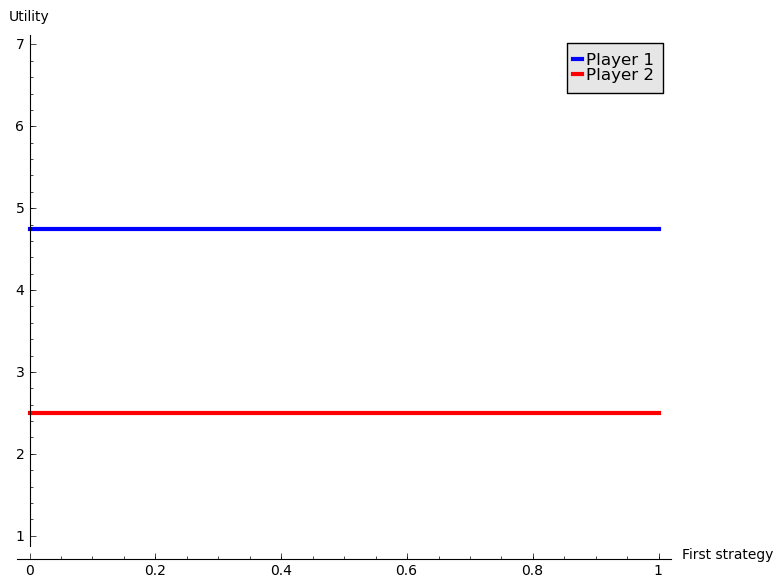
\includegraphics[width=8cm]{sage13.png}
\end{center}

$$u_1\approx4.8\text{ and }u_2\approx2.5$$

We can obtain the same results analytically:

$$\left.u_1=7\times q+4\times(1-q)\right|_{q={1\over4}}=4.75$$
$$\left.u_2=3\times p+2\times(1-p)\right|_{p={1\over2}}=2.5$$

\end{enumerate}

\end{document}
